\subsection*{Convergence and performance}

We verify spatial consistency by combining (i) field–norm error estimates on nested meshes with non-matching transfer, and (ii) \emph{quantity–of–interest} (QoI) Richardson analysis with Roache’s grid–convergence index (GCI). All quantities are nondimensional under the scaling in \S\ref{sec:strong-forms-nd}; averages are normalized by $|\Omega|$.

\paragraph{Meshes and notation.}
Let $\{\mathcal{T}_i\}_{i=1}^L$ be a family of tetrahedral meshes on $\Omega$ obtained by uniform refinement, with characteristic sizes $h_i=1/N_i$ (we report $h_i=1/N_i$ explicitly). On each $\mathcal{T}_i$ we solve the fully coupled problem to a fixed time $T$ with \emph{the same} $\Delta t$ and model parameters; this avoids additional time–discretization bias from remounting left–hand sides. Denote by
\[
\mathbf{u}_i,\quad S_i,\quad \rho_i,\quad \mathbf{A}_i
\]
the discrete fields on level $i$ in their conforming $H^1$ spaces $V_{h_i},Q_{h_i},Q_{h_i},T_{h_i}$. Because the solution can exhibit sharp internal layers (bone/void fronts), we do not assume high regularity.

\paragraph{Field–norm pair errors on the finer mesh.}
For two consecutive levels $(H,h)=(i,i{+}1)$ we evaluate errors on the finer mesh in a \emph{higher–order observation space}. For any field $X\in\{\mathbf{u},S,\rho,\mathbf{A}\}$ we construct $W_{h}^{(X)}$ by raising the polynomial degree by $\Delta p=2$, transfer $X_H$ to $W_{h}^{(X)}$ by non-matching interpolation, and interpolate the fine-field values into the same space. With $\mathcal{I}_{H\to h}$ denoting the non-matching interpolation and $\widetilde X_h$ the interpolated fine solution, the pair error reads
\[
e_{H\to h}^{X,\;L^2} \;=\; \big\| \widetilde X_h - \mathcal{I}_{H\to h} X_H \big\|_{L^2(\Omega)},
\qquad
e_{H\to h}^{X,\;H^1\text{-semi}} \;=\; \big\| \nabla(\widetilde X_h - \mathcal{I}_{H\to h} X_H) \big\|_{L^2(\Omega)} .
\]
Vector/tensor seminorms use the canonical componentwise sum. All integrals are evaluated with sixth-order quadrature on $\mathcal{T}_h$. For a sequence of pairs we obtain $\{(h_{i+1},e_{i\to i+1}^{X,\bullet})\}_{i=1}^{L-1}$ and estimate an experimental order of convergence (EOC) $p$ from the log–log fit
\[
\log e \approx p\,\log h + \mathrm{const},\qquad
p \;=\; \arg\min_{p} \sum_{i} \big(\log e_{i\to i+1}^{X,\bullet} - p\log h_{i+1} - c\big)^2 ,
\]
reported for both $L^2$ and $H^1$–semi norms. When only three levels are available, we also quote the two–ratio estimate $p \approx \log(e_{H\to h}/e_{h\to h/2})/\log(r)$ with $r=h_H/h_h$.

\paragraph{QoIs for convergence tracking.}
Alongside field norms we track scalar QoIs that remain robust for sharp solutions. The analysis reports
\[
\overline{u}_x \;=\; \frac{1}{|\Omega|}\int_\Omega \boldsymbol{u}\cdot\mathbf{e}_x\,\mathrm{d}x,\quad
\overline{S} \;=\; \frac{1}{|\Omega|}\int_\Omega S\,\mathrm{d}x,\quad
\overline{\rho} \;=\; \frac{1}{|\Omega|}\int_\Omega \rho\,\mathrm{d}x,\quad
\overline{\mathcal A} \;=\; \frac{1}{|\Omega|}\int_\Omega \mathrm{tr}(\mathbf A^{\top}\mathbf A)\,\mathrm{d}x,
\]
and the domain-average strain-energy density
\[
\overline{\psi} \;=\; \frac{1}{|\Omega|}\int_\Omega \tfrac12\,\boldsymbol{\sigma}(\mathbf{u},\rho,\mathbf{A}):\boldsymbol{\varepsilon}(\mathbf{u})\,\mathrm{d}x.
\]
The post-processing converts $\overline{u}_x$ to millimetres using the model scale $u_c$; all other quantities remain nondimensional unless stated otherwise.

\paragraph{QoI–based Richardson and GCI.}
Let $Q(h)$ be any scalar QoI from the set above. Using the last three levels $h_1>h_2>h_3$ (coarse$\to$fine) we form
\[
r_{21}=\frac{h_1}{h_2},\quad r_{32}=\frac{h_2}{h_3},\quad
d_{12}=Q(h_1)-Q(h_2),\quad d_{23}=Q(h_2)-Q(h_3).
\]
Assuming smooth asymptotics $Q(h)=Q_\infty + C h^p + o(h^p)$, the order and extrapolated limit are
\[
p \;=\; \bigg|\frac{\log|d_{12}/d_{23}|}{\log r_{21}}\bigg|,\qquad
Q_\infty \;\approx\; Q(h_3) + \frac{Q(h_3)-Q(h_2)}{r_{32}^{\,p}-1}.
\]
Following Roache, the (relative) GCIs between the last two spacings are
\[
\mathrm{GCI}_{21} \;=\; F_s\,\frac{|d_{12}|}{|Q(h_2)|}\,\frac{1}{|r_{21}^{\,p}-1|},\qquad
\mathrm{GCI}_{32} \;=\; F_s\,\frac{|d_{23}|}{|Q(h_3)|}\,\frac{1}{|r_{32}^{\,p}-1|},
\]
with safety factor $F_s=1.25$. We also report a monotonicity flag $\mathsf{mono}=\mathbb{1}[d_{12}d_{23}\ge 0]$ and the asymptoticity indicator
\[
\beta \;=\; \frac{|d_{12}|}{|d_{23}|}\,\frac{1}{\widehat r^{\,p}},\qquad
\widehat r = \begin{cases}
 r_{21}, & r_{21}=r_{32},\\
\dfrac{|h_2^{p}-h_1^{p}|}{|h_3^{p}-h_2^{p}|}, & \text{otherwise},
\end{cases}
\]
which matches the implementation used in the post-processing scripts. The indicator tends to $1$ when the last three levels are in the asymptotic range. For strongly localized solutions (as in our remodeling front), $p<1$ and $\beta\ll 1$ may legitimately occur; in that case the QoI averages ($\overline{\psi},\overline{\rho},\overline{S}$) provide the most informative trend.

\subsection*{Anisotropy index (QoI)}
For the fabric tensor $\mathbf A$ (symmetric, positive semidefinite, unit trace) we report the domain-average
\begin{equation*}
  \overline{\mathcal A} \;=\; \frac{1}{|\Omega|}\int_\Omega \mathrm{tr}\!\left(\mathbf A^{\!\top}\mathbf A\right)\,\mathrm d x,
\end{equation*}
i.e.\ the mean squared Frobenius norm of $\mathbf A$, which increases with anisotropy when $\mathrm{tr}\,\mathbf A=1$.

\paragraph{Implementation notes.}
Errors use DOLFINx non-matching transfer (creation of interpolation data on the fine grid and cell-wise interpolation), and all integrals are assembled with MPI reductions after updating ghost values. The same set of converged solutions $\{(\mathbf{u}_i,S_i,\rho_i,\mathbf{A}_i)\}$ is reused for field-norm and QoI analysis to avoid duplicating runs. Sixth-order quadrature suffices for the observation spaces employed here. Because we keep $\Delta t$ fixed across $h$ (no $h$-dependent remounting of left--hand sides), the study isolates \emph{spatial} sensitivity; in a posteriori checks on the finest mesh, halving $\Delta t$ changed the reported QoIs by less than our print precision, confirming that temporal error is subdominant in the regimes shown.

\paragraph{Reporting.}
We show (i) $h$ per level and per pair, (ii) EOC from the log–log fit for $L^2$ and $H^1$–semi norms of $(\mathbf{u},S,\rho,\mathbf{A})$, and (iii) for each QoI: $(p,Q_\infty,\mathrm{GCI}_{32},\beta,\mathsf{mono})$. Where relevant we additionally provide absolute GCIs (without normalization by $|Q(h)|$) to disambiguate small denominators.
\label{subsec:subsolver_conv}
\paragraph{Objective and approach}
We validate spatial and temporal consistency by comparing adjacent levels of mesh and time-step refinement. For each quantity we report (i) log--log error scaling versus $h$ and $\Delta t$, (ii) local pairwise orders of convergence, and (iii) solver performance scaling.

\begin{figure}[htbp]
  \centering
  \IfFileExists{images/convergence.png}{%
    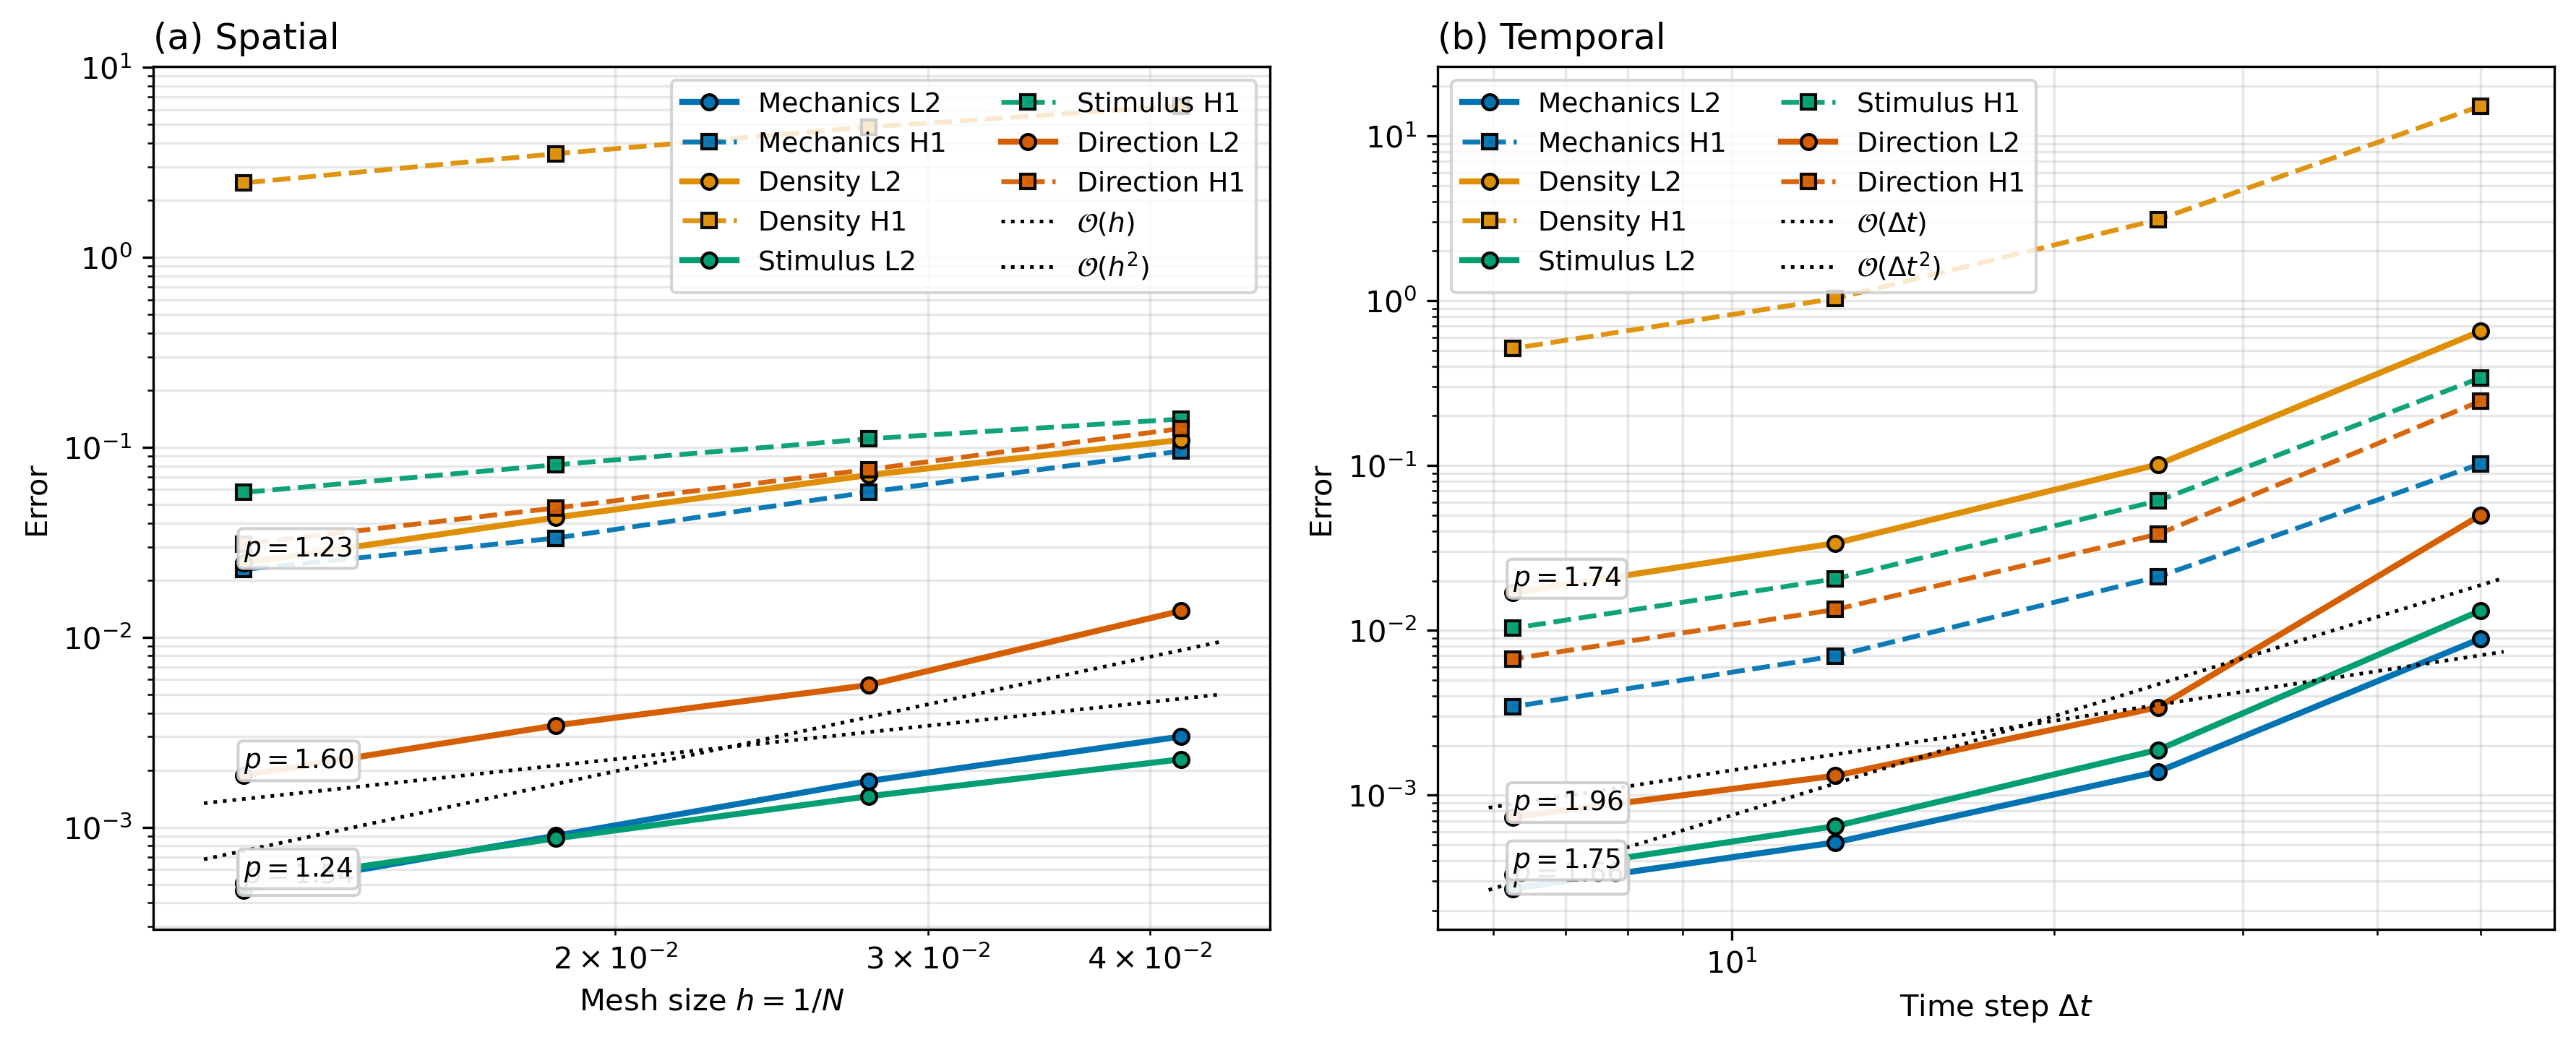
\includegraphics[width=0.92\linewidth]{images/convergence.png}%
  }{\fbox{\parbox{0.9\linewidth}{\centering Missing image: \texttt{images/convergence.png}}}}
  \caption{Convergence of spatial and temporal errors under mesh and time-step refinement. Solid lines: errors (norms specified in the text). Dotted lines: ideal slopes for $P^1$ elements and the Backward--Euler scheme. Shaded bands show interquartile ranges across regions of interest.}
  \label{fig:individual_convergence}
\end{figure}

\paragraph{Methodology}
Spatial errors compare consecutive meshes by interpolating both solutions into a higher-order observation space on the finer grid ($P^1\rightarrow P^3$) and evaluating $L^2$ and $H^1$ seminorms with sixth-order quadrature. Temporal errors reuse the same spatial discretization and contrast successive time steps. Local pairwise orders are estimated as
\begin{equation}
\begin{aligned}
p &\approx \frac{\log\big(\|e(h_i)\|/\|e(h_{i+1})\|\big)}{\log (h_i/h_{i+1})}, \\
q &\approx \frac{\log\big(\|e(\Delta t_j)\|/\|e(\Delta t_{j+1})\|\big)}{\log (\Delta t_j/\Delta t_{j+1})},
\end{aligned}
\end{equation}
with $e(\cdot)$ the successive differences and refinement ratios taken from the sweep metadata.

\paragraph{Spatial convergence}
At fixed $\Delta t$, errors decrease monotonically under mesh refinement and the pairwise orders approach the expected rates for $P^1$ elements. Local deviations near high gradients are consistent with limited smoothness and do not break the global trend (\cref{fig:individual_convergence}).

\paragraph{Temporal convergence}
As $\Delta t$ decreases, we observe a sublinear reduction in the earliest steps (transient adaptation), followed by the asymptotic first-order behavior of Backward--Euler.

\begin{figure}[htbp]
  \centering
  \IfFileExists{images/performance.png}{%
    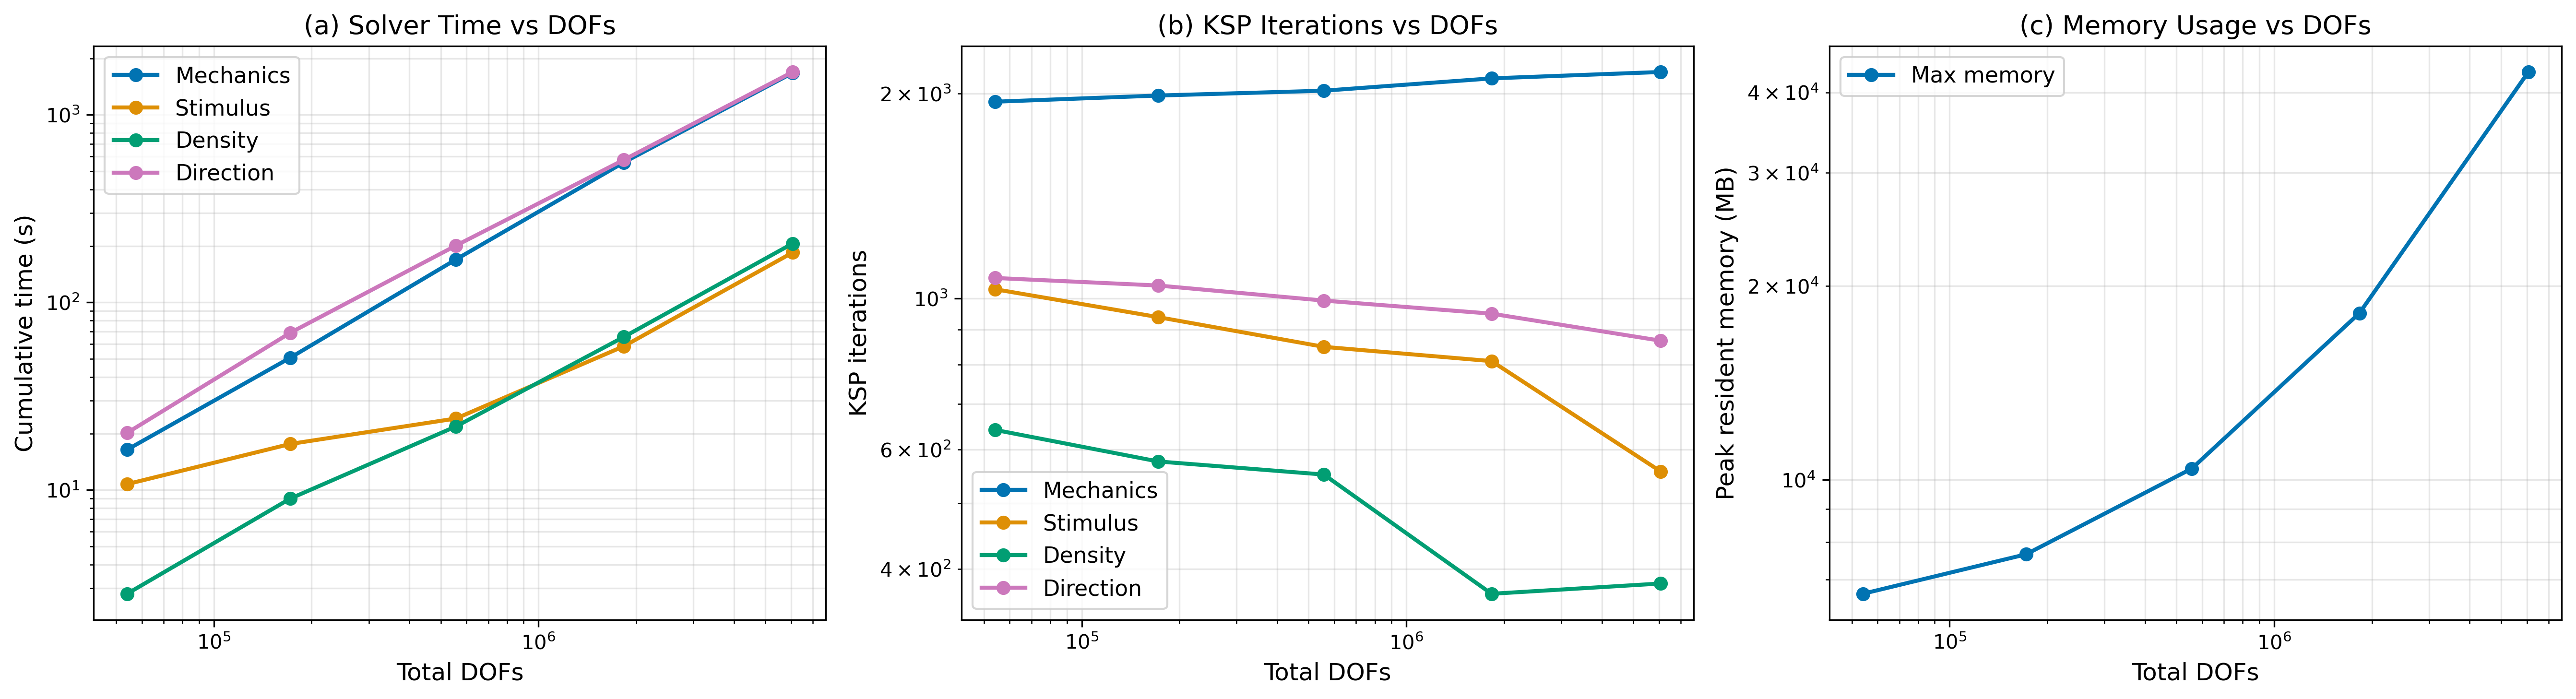
\includegraphics[width=1\linewidth]{images/performance.png}%
  }{\fbox{\parbox{0.9\linewidth}{\centering Missing image: \texttt{images/performance.png}}}}
  \caption{Solver performance: wall time per block iteration, memory footprint, and scaling with mesh size and $\Delta t$. Points show medians across steps; bands show interquartile ranges.}
  \label{fig:performance}
\end{figure}

\begin{table}[htbp]
  \centering
  \caption{Performance scaling summary for representative $\Delta t$. The exponent $\alpha$ is from a linear regression of $\log(\text{time})$ versus $\log(\text{DOF})$; larger $\alpha$ indicates worse scaling.}
  \label{tab:performance-scaling}
  \small
  \IfFileExists{tables/performance_scaling_dt_25_0.csv}{%
  \begin{adjustbox}{max width=\linewidth}
  \pgfplotstabletypeset[
    col sep=comma,
    every head row/.style={before row=\toprule, after row=\midrule},
    every last row/.style={after row=\bottomrule},
    columns/metric/.style={string type, column name={Metric}},
    columns/solver/.style={string type, column name={Solver}},
    columns/alpha/.style={column name={$\alpha$}, fixed, zerofill, precision=3},
    columns={metric, solver, alpha},
  ]{tables/performance_scaling_dt_25_0.csv}
  \end{adjustbox}
  }{}
\end{table}

\paragraph{Summary}
Both spatial and temporal refinement show the expected consistency and monotone error reduction. Solver costs correlate with coupling strength across fields; more strongly coupled steps increase the per-iteration cost and the benefits of AA-I (see \cref{subsec:anderson}). The tabulated metrics complement the figures with a compact numerical overview to aid replication.
